%%%%%%%%%%%%%%%%%%%%%%%%%%%%%%%%%%%%%%%%%%%%%%%%%%%%%%%%%%%%%%%%%%%%
% Trello API wrapper
%%%%%%%%%%%%%%%%%%%%%%%%%%%%%%%%%%%%%%%%%%%%%%%%%%%%%%%%%%%%%%%%%%%%

\chapter{Trello API wrapper}\index{Trello}\index{API}

These scripts fulfill very different tasks, but they have also much in common. For example almost every script loads single cards. At least potentially. So I wrote a set of functions and classes which represent Trello for Ruby. This is kind of a translation of Trello to Ruby and vice versa. Additionally now the scripts can use the functions and in consequence they can stay very lightweight and clean. Almost everything that's possible whith the Trello API is possible with this API wrapper, too. But it covers not all features, because the API is still in beta phase, so it changes quite quickly.

\begin{figure}[htb]
\centering
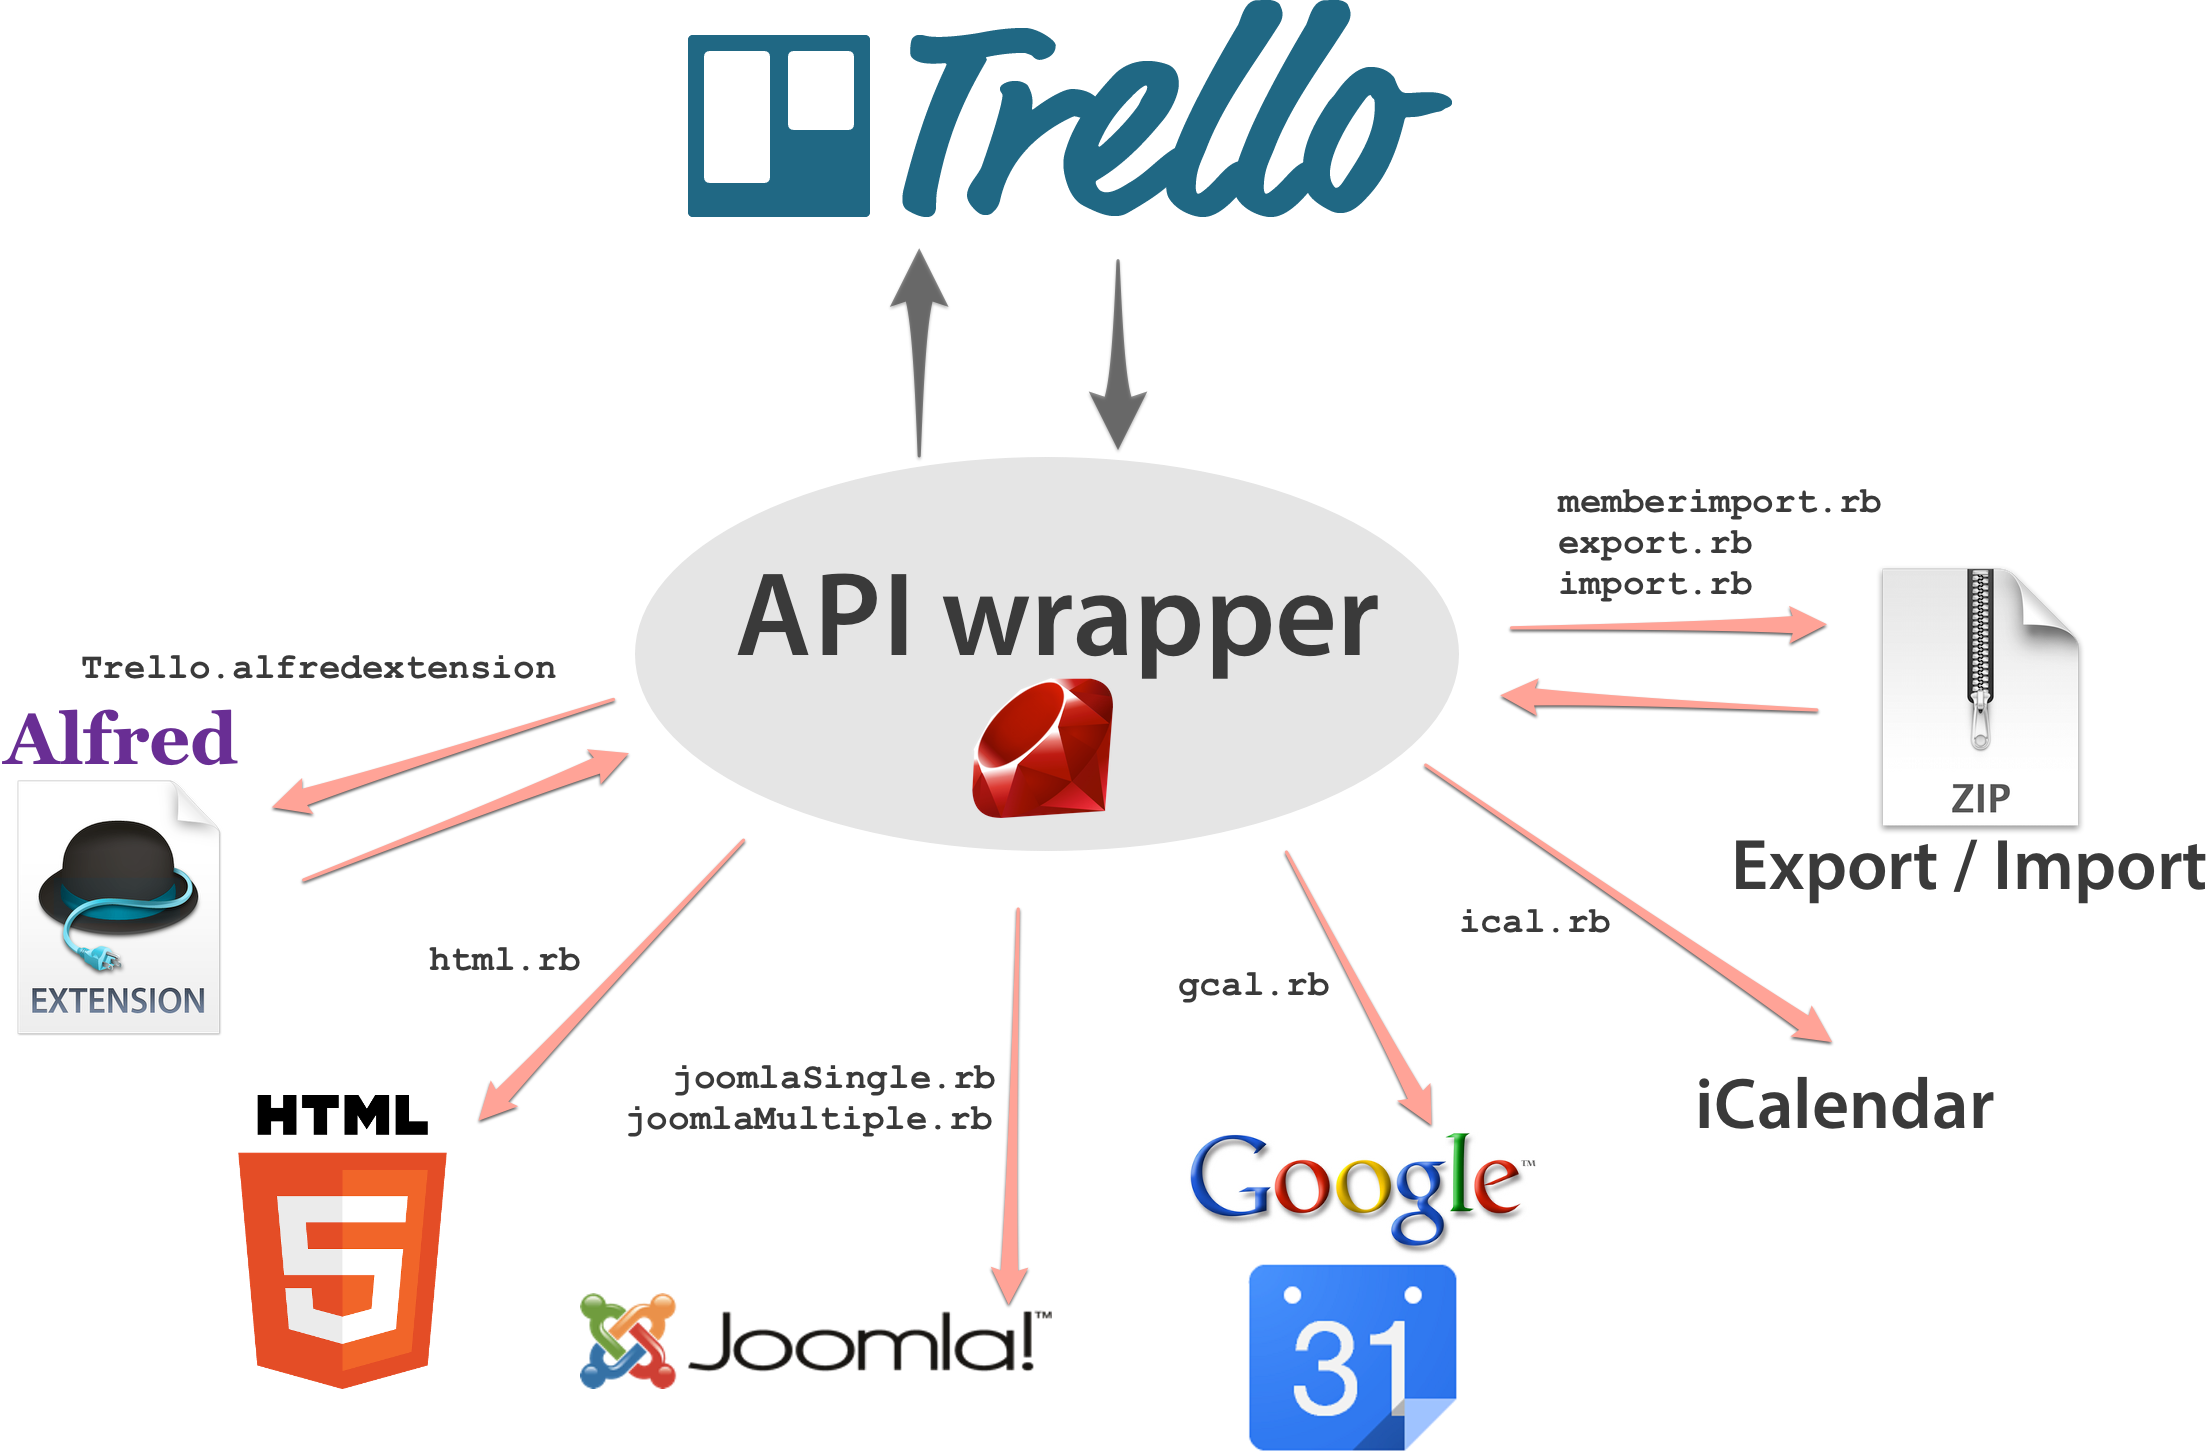
\includegraphics[width=\textwidth]{figures/api-wrapper}
\caption{Connections between Trello, the API wrapper and the actual features. \cite{ruby:icon}\cite{html:logo}\cite{joomla}\cite{google} }
\label{fig: api-wrapper}
\end{figure}

The API wrapper has also functions to pre-process data for Ruby. From a developers point of view, Trello is all about cards. Cards are the only things in Trello with real data, not just meta data. So if the task is so get a board from the API\index{API} it means to get the cards of the board. There is an API call to get all cards which are in a specific board. But with this call the developer doesn't get all information about the cards. So the API wrapper has to execute the API call for a single card to cummulate all information about all cards of the board. This is the function of the API wrapper to keep the actual script clean. So the developer can work with the data and hasn't to worry about determining them.

\todo{So stehen lassen?} The API wrapper is meant to perform all API calls which are required of the scripts. None of the API calls should be performed by the scripts that use the bucket.

\todo{MEHR! Wie unktioniert der wrapper?}

\todo{Die meisten gems im wrapper aufrufen}

\section{Error handling}
\todo{Error Handling}

\section{Command Line Interface}\nomenclature{CLI}{Command Line Interface}\index{CLI}\index{Command-Line Interface}\label{cli}
Almost every script needs some informations. An information which every scripts need is key and token of the user which account should be used for the access to Trello. The scripts have to know which cards, lists and boards they have to look at. So these information has to be passed to the scripts, too. At first we set this information at the top of the script. But it emerged that it's very unpractical to hard code this in each script. So it would be impossible to use the same Ruby file with several Trello accounts. For every Trello account the user has to generate a dedicated file. The solution for this problem is a command-line interface (CLI). With a CLI the user can pass information to the script in a predefined format, so the script knows exactly what to do. For every other call the user can specify different information for one and the same script.

The Ruby class OptionParser\cite{ruby:optionparser} provides easy customisable command-line option analysis. The developer is able to specify its own options for each script. For this purpose a dedicated class is used. 
In order to let the actual script \emph{know} about the CLI arguments the developer has to require the respective CLI class with the command-line option definitions.

\begin{lstlisting}[aboveskip=1\baselineskip, style=bash, caption=Example usage of a script with CLI., label=listing004]
ruby html.rb -c 4ffd78a2c063afeb066408b8
\end{lstlisting}

An example usage of a script with CLI would look like Listing \ref{listing004}. The \texttt{-c} is an comman-line option. If there is a string behind the option, like in this case, the string is a so called \emph{argument}. But there are command-line options which stand for its own. Those are called \emph{flags}. Flags are only for polar decisions.

\begin{lstlisting}[aboveskip=1\baselineskip, caption=Definition of a command-line option, label=listing002]
# Trello list(s)
opts.on("-l", "--lists x,y,z", Array, "Ids of one or more Trello lists.") do |lists| (*@\label{line001}@*)
	options.lists = lists
end
\end{lstlisting}

Listing \ref{listing002} shows the definition of the option \texttt{-l} for passing one or more IDs of lists to a script. In Line \ref{line001} the word \lstinline{Array} casts the list argument to an Array object.

OptionParse provides an automated help option. If the user types 
\begin{center}
\texttt{ruby script.rb -h} 
\end{center}
he gets the explanation the developer wrote in the CLI class for this script with all possible options. This list ist automatically generated by the definitions of the command-line options like in Listing \ref{listing002}. It works with \texttt{-help} and \texttt{--help} instead of \texttt{-h}, too.

\begin{lstlisting}[aboveskip=1\baselineskip, style=bash, caption=Output of the \texttt{-h} option., label=listing003]
Usage: ical.rb [options]
Select the input cards with -c, -l, -b or -a

Specific options:
 -a, --[no-]all         Set this if all due dates of all cards of all boards this user can see shall be used.
 -l, --lists x,y,z      Ids of one or more Trello lists.
 -b, --boards x,y,z     Ids of one or more Trello boards.
 -c, --cards x,y,z      Ids of one or more Trello cards.
 -k MANDATORY, --key    Your Trello key.
 -t MANDATORY, --token  The Trello token.
\end{lstlisting}

Listing \ref{listing003} shows the Output of \texttt{ruby ical.rb -h}. 
These are the basic CLI commands used by every script. For some scripts there are additional commands. They are explained in their respective sections.

\section{Handling of date and time}
The cards in Trello may have set due dates. A due date is a date at which the creator of the card thinks it should be done. The due date is represented by the Trello API as an ISO\nomenclature{ISO}{International Organization for Standardization} 8601\index{ISO!8601} formatted string. The timezone\index{timezone} of the date is UTC\nomenclature{UTC}{Universal Time Coordinated}. To ensure that the correct time is displayed always the date has to be adapted to the local time. That's perfeormed with the code in listing \ref{listing021}.

\begin{lstlisting}[aboveskip=1\baselineskip, caption=Response of the token request., label=listing021]
fdate = Time.iso8601(date).getlocal
\end{lstlisting}

It parses the given date string in ISO 8601 format to a Ruby Time object. The \lstinline{getlocal} is the important part here. This function of the Time class determines server's time zone and readjusts the time accordingly. The method respects the daylight saving time applay in several time zones, too. For this function working as intended it's important that the correct time zone is set on the used server. 

\subsection{getDate(date, format='de')}

\todo{Describe getDate}

\section{Collect data from Trello}

\todo{Describe all the methods. Consider renaming for constancy?}

\section{Further information on a card}

\todo{Describe all the methods. Consider renaming for constancy?}

\section{Member information}

\subsection{getMember(memberId)}

\subsection{isThisMe(memberId)}

\section{Accessing CMS}

\subsection{trelloJoomlaSync(cardId, sectionid, catid, joomlaVersion)}




